% In this talk, I’ll talk about how we can use silly games to understand the strengths and weaknesses of AIs. We first begin with games that test memory: testing the recall of obscure facts. While AI has been viewed as superhuman at this task, it isn’t universally so. We show that a new measure of adversarial datasets (the gap between humans and computers) is decreasing but not yet closed, with computers still struggling on abstract reasoning and knowing when they know the correct answer. Given these disparate skill sets, we then analyze how we can best build human and computer teams ito learn new facts and detect false statements. Finally, I close with a similar line of results for another silly language game, Diplomacy, where computers have still not reached dominance but can be used to assist human players think strategically and detect lies.”

\documentclass[compress]{beamer}

%\usepackage{beamerthemesplit}
\usepackage{xmpmulti}

\usepackage{booktabs}
\usepackage{graphicx,float,wrapfig, bbm}
\usepackage{amsfonts, bbold, comment}
\usepackage{mdwlist}
\usepackage{subfigure}
\usepackage{colortbl}
\usepackage{overpic}
\usepackage{pdfpages}
\usepackage[normalem]{ulem}
\usepackage{multirow}

\pgfdeclareimage[width=\paperwidth]{mybackground}{../../common/boulder.pdf}

\newcommand{\advscore}{\abr{AdvScore}}
\newcommand{\tif}[0]{\abr{tif}}
\newcommand{\twoplprob}[3]{ \frac{1}{\ex{-#3\left[ #1 - #2 \right] }  }}
\newcommand{\iif}{\abr{iif}}
\newcommand{\slda}[0]{\abr{slda}}
\newcommand{\bm}[1]{\mbox{\boldmath$#1$}}
\newcommand{\lda}[0]{\abr{lda}}
\newcommand{\explain}[2]{\underbrace{#2}_{\mbox{\footnotesize{#1}}}}
\newcommand{\itmspace}[0]{\hspace{2cm}}
\newcommand{\pos}[1]{{\texttt{#1}}}
\newcommand{\e}[2]{\mathbb{E}_{#1}\left[ #2 \right] }
\newcommand{\ind}[1]{\mathbb{I}\left[ #1 \right] }
\newcommand{\abr}[1]{\textsc{#1} }
\newcommand{\ex}[1]{\mbox{exp}\left\{ #1\right\} }
\newcommand{\g}{\, | \,}
\newcommand{\citename}[1]{#1 }
\newcommand{\fsi}[2]{
\begin{frame}[plain]
\vspace*{-1pt}
\makebox[\linewidth]{\includegraphics[width=\paperwidth]{#1}}
\begin{center}
#2
\end{center}
\end{frame}
}


\newcommand{\danquote}[1]{

\begin{flushright}
\begin{overpic}[width=5.5cm,tics=10]{general_figures/speech_bubble}
	\put(10,30) { \parbox{4cm}{#1 }}
\end{overpic}

\includegraphics[width=1.5cm]{general_figures/milkman_dan}
\end{flushright}
}


\newcommand{\gfxd}[2]{
	\begin{center}
		\includegraphics[width=#2\linewidth]{diplomacy/#1}
	\end{center}
}

\newcommand{\gfxt}[2]{
\begin{center}
	\includegraphics[width=#2\linewidth]{reading_tea_leaves/#1}
\end{center}
}

\newcommand{\gfxi}[2]{
\begin{center}
	\includegraphics[width=#2\linewidth]{interpretability/#1}
\end{center}
}

\newcommand{\gfxs}[2]{
\begin{center}
	\includegraphics[width=#2\linewidth]{simtrans/#1}
\end{center}
}

\newcommand{\gfxq}[2]{
\begin{center}
	\includegraphics[width=#2\linewidth]{qb/#1}
\end{center}
}


\newcommand{\gfxa}[2]{
	\begin{center}
		\includegraphics[width=#2\linewidth]{advcal/#1}
	\end{center}
}


\newcommand{\gfxu}[2]{
	\begin{center}
		\includegraphics[width=#2\linewidth]{uncertainty/#1}
	\end{center}
}

\newif\ifjobtalk\jobtalktrue
\newif\iflong\longtrue

\usetheme[
          showdate=true,                     % show the date on the title page
          alternativetitlepage=true,         % Use the fancy title page.
          titlepagelogo=general_figures/shell,              % Logo for the fir\
st page.
          ]{UMD}


\title[]{Computers and Humans Playing Language Games Together}
\author{ Jordan Boyd-Graber}
\date{2025}

\institute[] % (optional, but mostly needed)
{University of Maryland}


%gets rid of bottom navigation symbols
\setbeamertemplate{navigation symbols}{}

%gets rid of footer
%will override 'frame number' instruction above
%comment out to revert to previous/default definitions
\setbeamertemplate{footline}{}

\begin{document}

\frame{
\titlepage
\tiny
}


\begin{frame}{Why Language Games?}


  \begin{columns}


    \column{.5\linewidth}
    \gfxa{wittgenstein}{.8}


    \column{.5\linewidth}


    \begin{itemize}

      \item Wittgenstein: Language is a product of the context in which it is
        used
      \item Interaction allows us to figure out how to use language
        \item Score lets us know how well we're doing
    \end{itemize}


    \end{columns}

  

\end{frame}

\fsi{qb/starcraft}{Image: DeepMind}
\fsi{qb/DeepBlue}{Peter Morgan/Reuters}

\begin{frame}{Today's Takeaways}
	\begin{itemize}
	\item Different Systems and Skilled Humans have Different Strengths
	\begin{itemize}
		\item Retrieval Methods: Less likely to confabulate
		\item LLMs: Good for easy, straightforward tasks
		\item Humans: good for nuance and abstraction
	\end{itemize}
	\item It takes work to figure this out
	\begin{itemize}
		\item Getting harder examples
		\item Measuring human vs. computer accuracy: Item Response Theory
                \item Competitive and Cooperative
	\end{itemize}
	\item Tasks
	\begin{itemize}
		\item Finding false claims
		\item Question answering
		\item Detecting lies
	\end{itemize}
	\end{itemize}
\end{frame}

\begin{frame}{Fact Checking with Humans in the Loop}
	\begin{columns}
		\column{.5\linewidth}

\gfxu{paper_convincingly}{.9}

\column{.5\linewidth}
\begin{center}
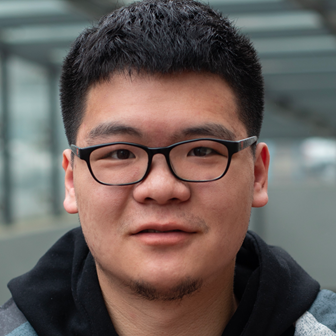
\includegraphics[width=1.0\linewidth]{general_figures/chenglei}		
	
\end{center}
	\end{columns}
\end{frame}

\begin{frame}{Research Questions}
	\begin{itemize}
		\item Are natural language explanations more effective than retrieved passages for human fact-checking?
		\item Can contrastive explanations—arguing for or against a fact being true—mitigate over-reliance and be more effective than non- contrastive explanations?
		\item  Are there complementary benefits in presenting both natural language explanations and retrieved passages?
	\end{itemize}
\end{frame}
 
  \fsi{uncertainty/fever}{\textbf{F}act \textbf{E}xtraction and \textbf{VER}ification}
  		
\begin{frame}{FEVER categories}
	\begin{itemize}
		\item Examples from FEVER (Thorne et al., 2018)
		\item Supported:
		\begin{itemize}
			\item Woody Allen is a person.
			\item The Shining was directed.
			\item François de Belleforest wrote.
		\end{itemize}
		\item \alert<2>{Not Enough Info}:
		\begin{itemize}
			\item Lisa Kudrow was in a car.
			\item Tipper Gore was curated to Al Gore.
			\item International Relations includes animals.
		\end{itemize}
		\item Refuted:
		\begin{itemize}
			\item Tipper Gore was created in 1048.
			\item Alpha House is inspired by nobody.
			\item Toy Story is incapable of being a film.
		\end{itemize}
	\end{itemize}
	You don't always need the evidence
	(Poliak, 2018)
\end{frame}

\begin{frame}{Fool Me Twice}
	\gfxu{fm2}{1.0}
\end{frame}

\begin{frame}{Author Claims where Gold Evidence is \textbf{not} Model's Top Evidence}
	\only<1>{\gfxu{fm2_interface_0}{.9}}
	\only<2>{\gfxu{fm2_interface_1}{.9}}
	\only<3>{\gfxu{fm2_interface_2}{.9}}
	\only<4>{\gfxu{fm2_interface_3}{.9}}
	\only<5>{\gfxu{fm2_interface_4}{.9}}				
\end{frame}

% TODO(jbg): Add Fm2 screenshots

\begin{frame}{It is Harder (a bit)}
	\gfxu{fm2_retrieval}{.8}
\end{frame}

\begin{frame}{Claim: Manhattan has the most residents of New York City's boroughs. }
	\begin{columns}
		\column{.5\linewidth}
	\begin{block}{Direct}
		 \scriptsize The claim that Manhattan has the most residents of New York City's boroughs is false.  Manhattan has a population of approximately 1.6 million residents. However, New York City as a whole has a population of approximately 8.3 million residents. Therefore, Manhattan does not have the most residents among New York City's boroughs.  
    \end{block}

		\begin{block}{Case For}
			\scriptsize
		Manhattan is the most populous borough in New York City, with a population of approximately 1,627,788 as of 2025.  The other boroughs have smaller populations: Brooklyn: 2.72 million; Queens: 2.57 million; The Bronx: 1.46 million; Staten Island: 552,00.
	\end{block}	
    
		\column{.5\linewidth}	

    
    	\begin{block}{IR}
    	 \scriptsize New York City's borough of Manhattan is the highest nominal income county in the United States. In particular, ZIP code 10021 on Manhattan's Upper East Side, with more than 100,000 inhabitants and a per capita income of over \$90,000, has one of the largest concentrations of income in the United States. The other boroughs, especially Queens and Staten Island, have large middle-class populations. 
    \end{block}


		\begin{block}{Case Against}
			\scriptsize According to recent data, Brooklyn is the most populated borough in New York City, not Manhattan. Manhattan has a population of approximately 1.6 million residents, while Brooklyn has a significantly higher population.
		\end{block}					
	\end{columns}
		
		
\end{frame}


\begin{frame}{Results}
	\begin{columns}
		\column{.5\linewidth}
		\gfxu{acc_correct}{1.0}
		\column{.5\linewidth}
		\only<2>{\gfxu{acc_wrong}{1.0}}
	\end{columns}
\end{frame}

\begin{frame}{Why not just show IR all the time?}
	\pause
	\gfxu{time}{.5}
\end{frame}

\begin{frame}{Breaking Things Down}
	\begin{itemize}
	\item What's the solution?
	\item If the models were never wrong, we wouldn't have this problem
	\item If the models could know when they were wrong, we wouldn't have this problem
	\item \alert<2->{If we knew when the models would be wrong, we wouldn't have this problem}
	\end{itemize} 
	\begin{block}{CAIMIRA}
		Model that can predict when a model is likely to get a question right
	\end{block}
\end{frame}

\begin{frame}{CAIMIRA}
	\gfxa{paper_caimira}{1.0}
	\begin{center}
		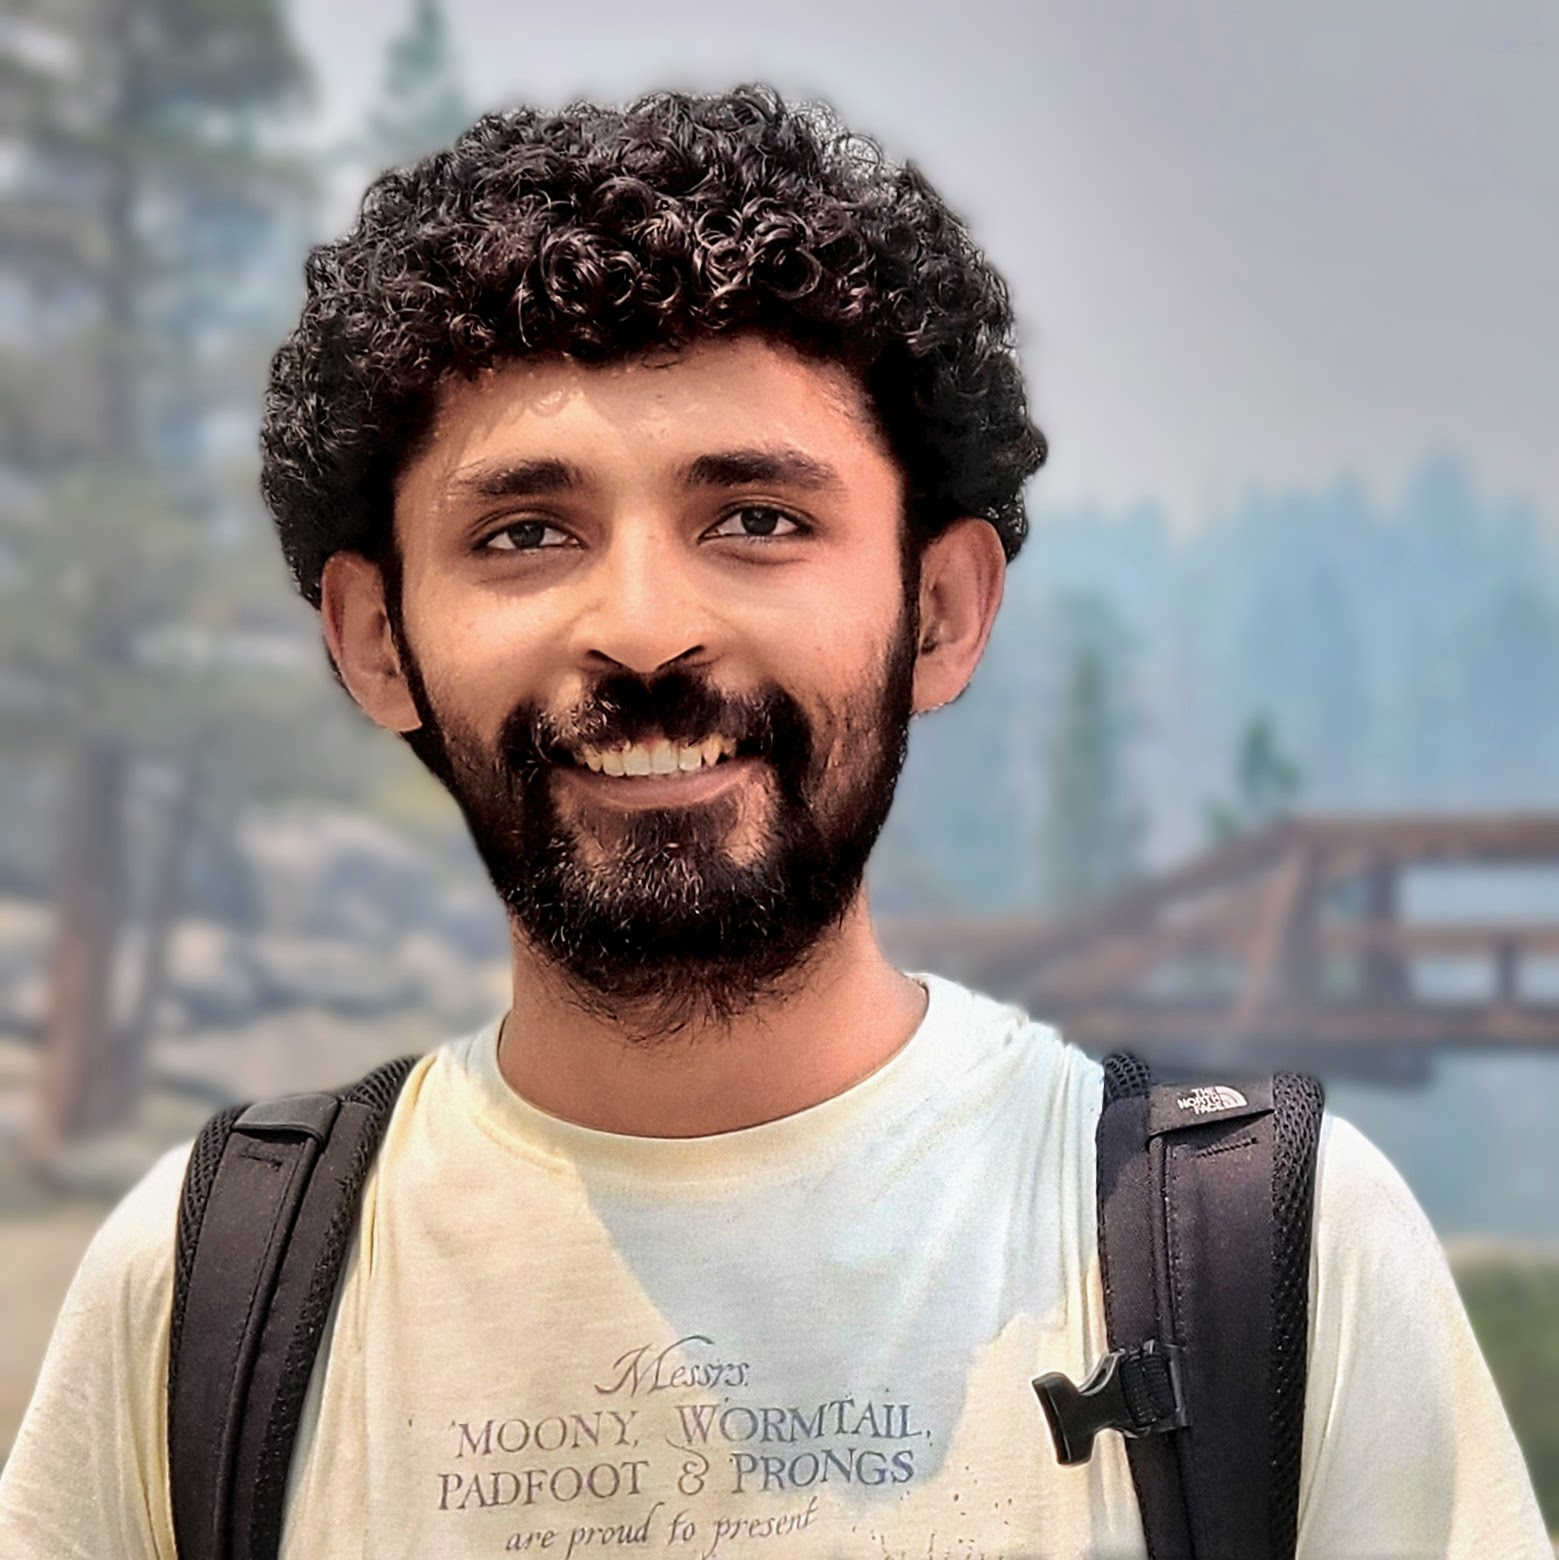
\includegraphics[width=0.25\linewidth]{general_figures/maharshi}
	\end{center}
\end{frame}


%todo(jbg):  or irt and chimera

\begin{frame}{Item Response Theory}

\only<1>{\gfxa{sat_sheet}{.9}}
\only<2>{\gfxa{sat_sheet_prob}{.9}}


\only<3>{\gfxa{jeopardy_irt_0}{.7}}
\only<4>{\gfxa{jeopardy_irt_1}{.7}}
\only<5>{\gfxa{jeopardy_irt_2}{.7}}

\end{frame}


  \begin{frame}{Making Dimensions Interpretable}
    % TODO(jbg): Add equations
        \begin{itemize}
        \item Make skills and difficulty vector-valued
          \begin{equation}
            \gamma_j \sum_k \left[ \theta_{i,k} - \beta_{j,k} \right]
          \end{equation}
        \item Where do the dimensions come from?
          \pause
          \begin{itemize}
          \item Latent variable: learned to predict correctness
          \item Function of question encoding, question features
          \item Regularized to be sparse
          \end{itemize}
    \item Posthoc labeling
    \end{itemize}
	\gfxq{caimira_component}{.5}
 \end{frame}

  \begin{frame}{Hard for Computers: Abductive Inference}

    \begin{columns}
      \column{.5\linewidth}
      \gfxa{caimira_abductive_features}{1.0}
      \column{.5\linewidth}      
      \only<2>{\gfxa{caimira_abductive_skills}{1.0}}
    \end{columns}

  \end{frame}


  
  \begin{frame}{Hard for Humans: Science}

    \begin{columns}
      \column{.5\linewidth}
      \gfxa{caimira_science_features}{1.0}
      \column{.5\linewidth}      
      \only<2>{\gfxa{caimira_science_skills}{1.0}}
    \end{columns}

  \end{frame}

  \begin{frame}{Adversarial Datasets}

    \begin{columns}
      \column{.5\linewidth}
      \gfxq{benchmark_saturation}{1.0}
            \column{.5\linewidth}
            \begin{itemize}
            \item Biggio et al., 2012: Poisoning attacks against Support Vector Machines

              \gfx{adversarial_turtle}{.6}
              %TODO(jbg): add adversarial citation
              
            \item Many benchmarks are ``saturated''
            \item Newer datasets claim to be ``adversarial''
              \begin{itemize}
              \item Hard for computers, ``easy'' for humans
              \item No real metric / definition
              \end{itemize}
            \item Can we use the lessons of the previous paper to inform how to write hard examples
            \item Can we \emph{measure} how well we did?
              \pause
            \item Language game: increasing the difficulty level
              \item But need to measure!
    \end{itemize}
            \end{columns}
 \end{frame}

    \begin{frame}{Expanding IRT: Discriminability}

    \gfxq{discrimination}{1.0}

      \end{frame}
    
    \begin{frame}{Finding Skill of Subject is Like Binary Search}
    	\only<1>{\gfxq{discrimination_1}{1.0}}
    	\only<2>{\gfxq{discrimination_2}{1.0}}
    	\only<3>{\gfxq{discrimination_3}{1.0}}
    	\only<4>{\gfxq{discrimination_4}{1.0}}
    	\only<5>{\gfxq{discrimination_5}{1.0}}
    \end{frame}
    
    \begin{frame}{Adversarial Score}


\only<6->{
	\vspace{-1.5cm}
	\begin{block}{Adversarial Score}
		
		\begin{equation}
			\text{\advscore{}}_\text{j} = \frac{\mu_j}{1 + \delta_j} \cdot (1 + \kappa_j)
		\end{equation}
		
		
	\end{block}
	
	
}


      \begin{itemize}
      \item Use \abr{irt} again
        \item Model probability of skilled human getting it right, compare to models (want it to be high!)
\begin{equation}\label{eq:margin}
    \mu_j = \explain{Skilled human rep. prob.}{\twoplprob{\beta^{H_{(0)}}_{*}}{\theta_j}{\gamma_j}} - \explain{Skilled model rep. prob.}{\twoplprob{\beta^{M_{(0)}}_{*}}{\theta_j}{\gamma_j}},
\end{equation}
\only<2>{
  \begin{block}{Why not use raw accuracy?}
    \begin{itemize}
    \item Want patterns, not luck
    \item \abr{irt} can find (and downweight) bad questions
    \end{itemize}
  \end{block}

}
\only<3->{
\item Skilled humans should agree on the answer
  \begin{equation}\label{eq:delta}
    \delta_j = \sum_{i \sim H_{(1)}}
    \left[
      \frac{\twoplprob{\beta_i^{H_{(1)}}}{\theta_j}{\gamma_j} -
        \bar{p_{H_{(1)}}(r_{i,j})}}
           {|H_{(1)}|}
    \right].
\end{equation}
}

\only<4->{
  \item Question should be informative (Fischer information to agent skill):
\begin{align}\label{eq:iif}
\only<4>{\iif{}_j(\theta) &= \gamma_j^2  \cdot p_j(\theta) \cdot (1 -p_j(\theta)), \text{ where} \\
p_j(\theta) &= \twoplprob{\theta}{\theta_j}{\gamma_j}}
    \kappa_j &= 1-\exp\left(-{\tif{}_j}\right).
\end{align}

}

\end{itemize}
      
    \end{frame}

    \begin{frame}{AdvQA: Is this a viable incentive structure?}
      \begin{itemize}
    \item Can human authors interpret incentive?
      \begin{itemize}
      \item Computers should get questions wrong, smart humans should get them right
      \item Answers should be unique and easily verifiable
      \item Reward knowledge and skill
        \item Avoid ambiguity
      \end{itemize}
    \item Posthoc (no realtime feedback): Prizes given based on metric
      \item Professional trivia writers
      \end{itemize}
   \end{frame}
   
   
   \begin{frame}{What makes for Adversarial Example}
   	\only<1>{\gfxa{irtplot_0}{.9}}	
   	\only<2>{\gfxa{irtplot_1}{.9}}
   	\only<3>{\gfxa{irtplot_2}{.9}}
   	\only<4>{\gfxa{irtplot_3}{.9}}
   	\only<5>{\gfxa{irtplot_4}{.9}}
   	\only<6>{\gfxa{irtplot_5}{.9}}
   	\only<7>{\gfxa{irtplot_6}{.9}}
   \end{frame}

\begin{frame}{Adversarial Strategies}
	\begin{columns}
		\column{.5\linewidth}
			\only<1-2>{\gfxa{chrisrock}{.9}}
			\only<3-4>{\gfxa{parasite}{.9}}
		\column{.5\linewidth}
			\only<1-2>{What is the name of the American actor who stood up for his wife with a "slap that was heard around the world" during a popular awards show?}
			\only<2>{\\ \textbf{Brad Pitt / Will Smith}}
			\only<3-4>{What post-apocalyptic film directed by a Korean but not the director of Parasite is an allegory set on a train featuring the machinations of a rich businessman against the occupants of other cars?}
			\only<4>{\\ \textbf{Snowpiercer / Train to Busan}		}
	\end{columns}
\end{frame}

    
    % TODO(jbg): AdvCal Picture slide

    \begin{frame}{Which Datasets are Adversarial?}
      \gfxa{cumulative_advscore}{.9}

      \begin{itemize}
      \item Not all datasets remain adversarial forever
      \item What helps make datasets adversarial?
        \begin{itemize}
          \item Bamboogle: Automatically generated          
          \item TrickMe: Human in the loop interface (expert), \abr{ir} models
        \item FM2: Human in the loop interface (crowdworker), \abr{ir} models
        \item AdvQA: Huaman in the loop (expert), \abr{llm} model + category instructions
        \end{itemize}

      \end{itemize}
    \end{frame}

\fsi{simtrans/centaur-chess}{Centaur Chess}

\fsi{qb/augment/screenshot_all}{Interface}

\fsi{qb/augment/screenshot_guesses}{}

\fsi{qb/augment/screenshot_highlight}{{\bf Highlighting}}

\fsi{qb/augment/screenshot_evidence}{}

\begin{frame}{Experts vs. Novices}

 \begin{block}{Experts}
   Trivia experts, familiar with task, enjoy the task
 \end{block}

 \begin{block}{Mechanical Turkers}
   Mechanical Turkers: easily overwhelmed, need the help
 \end{block}

\end{frame}

\fsi{qb/augment/tools_acc}{Evidence helps novices, experts are expert}
% \fsi{qb/augment/tools_buzz}{Highlights help experts}

\begin{frame}{Skill Boost}
  Rerun IRT analysis: rather than contrast human vs. computer skill,
  we see how much interface boosts (or diminishes) user skill.
    \pause

    \begin{block}{Coefficients tell story!}
      \begin{itemize}
        \item {\bf Big, Positive}: Help
        \item {\bf Big, Negative}: Hurt
        \item {\bf Small}: Neutral
      \end{itemize}
    \end{block}

\end{frame}


\fsi{qb/augment/coefs_0}{Everything helps: Evidence for novies,
  Highlight for experts}
\fsi{qb/augment/coefs_1}{Synergistic effects}
\fsi{qb/augment/coefs_2}{Highlight and evidence help experts most}
\fsi{qb/augment/coefs_3}{For novices, less synergy}


\begin{frame}{}

  \begin{columns}
    \column{.4\linewidth}
    \begin{center}
        
\includegraphics[width=0.8\linewidth]{general_figures/shi}
        \end{center}
    \column{.6\linewidth}
    \begin{block}{\href{http://umiacs.umd.edu/~jbg//docs/2023_emnlp_augment.pdf}{Learning to Explain Selectively}}
      \underline{\href{http://users.umiacs.umd.edu/~shifeng/}{Shi Feng}} and {\bf Jordan Boyd-Graber}.  \emph{Empirical Methods in Natural Language Processing}, 2022
        \end{block}

  \end{columns}
\end{frame}


\begin{frame}{Measuring Interpretability}

  \only<1>{\gfxq{qb_centaur_1}{.9}}
  \only<2>{\gfxq{qb_centaur_2}{.9}}
  \only<3>{\gfxq{qb_centaur_3}{.9}}
  \only<4>{\gfxq{qb_centaur_6}{.9}}


\end{frame}




\begin{frame}{Improvement through Bandit Algorithms}

  \only<1>{\gfxq{rl_centaur_2}{.9}}
  \only<2>{\gfxq{rl_centaur_3}{.9}}
  \only<3>{\gfxq{rl_centaur_4}{.9}}
  \only<4>{\gfxq{rl_centaur_5}{.9}}
  \only<5>{\gfxq{rl_centaur_6}{.9}}

  \only<5->{Bandit actions~\cite{robbins-52}: turn each of the explanations (Guess,
    Highlight, Evidence) on or off.}
\end{frame}

\fsi{qb/augment/bandit_result_none}{Human alone without an AI teammate}
\fsi{qb/augment/bandit_result_ai}{AI alone without a human teammate}
\fsi{qb/augment/bandit_result_dynamic}{Dynamic assistance to human}
\fsi{qb/augment/bandit_result}{Better than showing everything!}

    

\begin{frame}{Changing Gears}

\begin{columns}
	
	\column{.5\linewidth}
	\gfxd{cicero_science}{1.0}
	\column{.5\linewidth}	
\begin{itemize}
	\item Focusing on interpersonal relationships
\begin{itemize}
	\item Cooperation
	\item Deception
	\item Betrayal
\end{itemize}
\item Multi-turn interactions
\end{itemize}

\end{columns}


\end{frame}

\begin{frame}{}
	
	\begin{columns}
		\column{.5\linewidth}
		
\includegraphics[width=0.7\linewidth]{general_figures/vlad}
		\column{.5\linewidth}
		\begin{block}{{\bf
					\href{http://cs.colorado.edu/~jbg//docs/2015_acl_diplomacy.pdf}{Linguistic Harbingers of Betrayal: A Case Study on an Online Strategy Game}}}
			
			Vlad Niculae, Srijan Kumar, Jordan Boyd-Graber, and Cristian
			Danescu-Niculescu-Mizil. \emph{Association for Computational Linguistics}, 2015
		\end{block}
		
	\end{columns}
\end{frame}


\begin{frame}[plain]
	\vspace*{-1pt}
	\only<1>{\makebox[\linewidth]{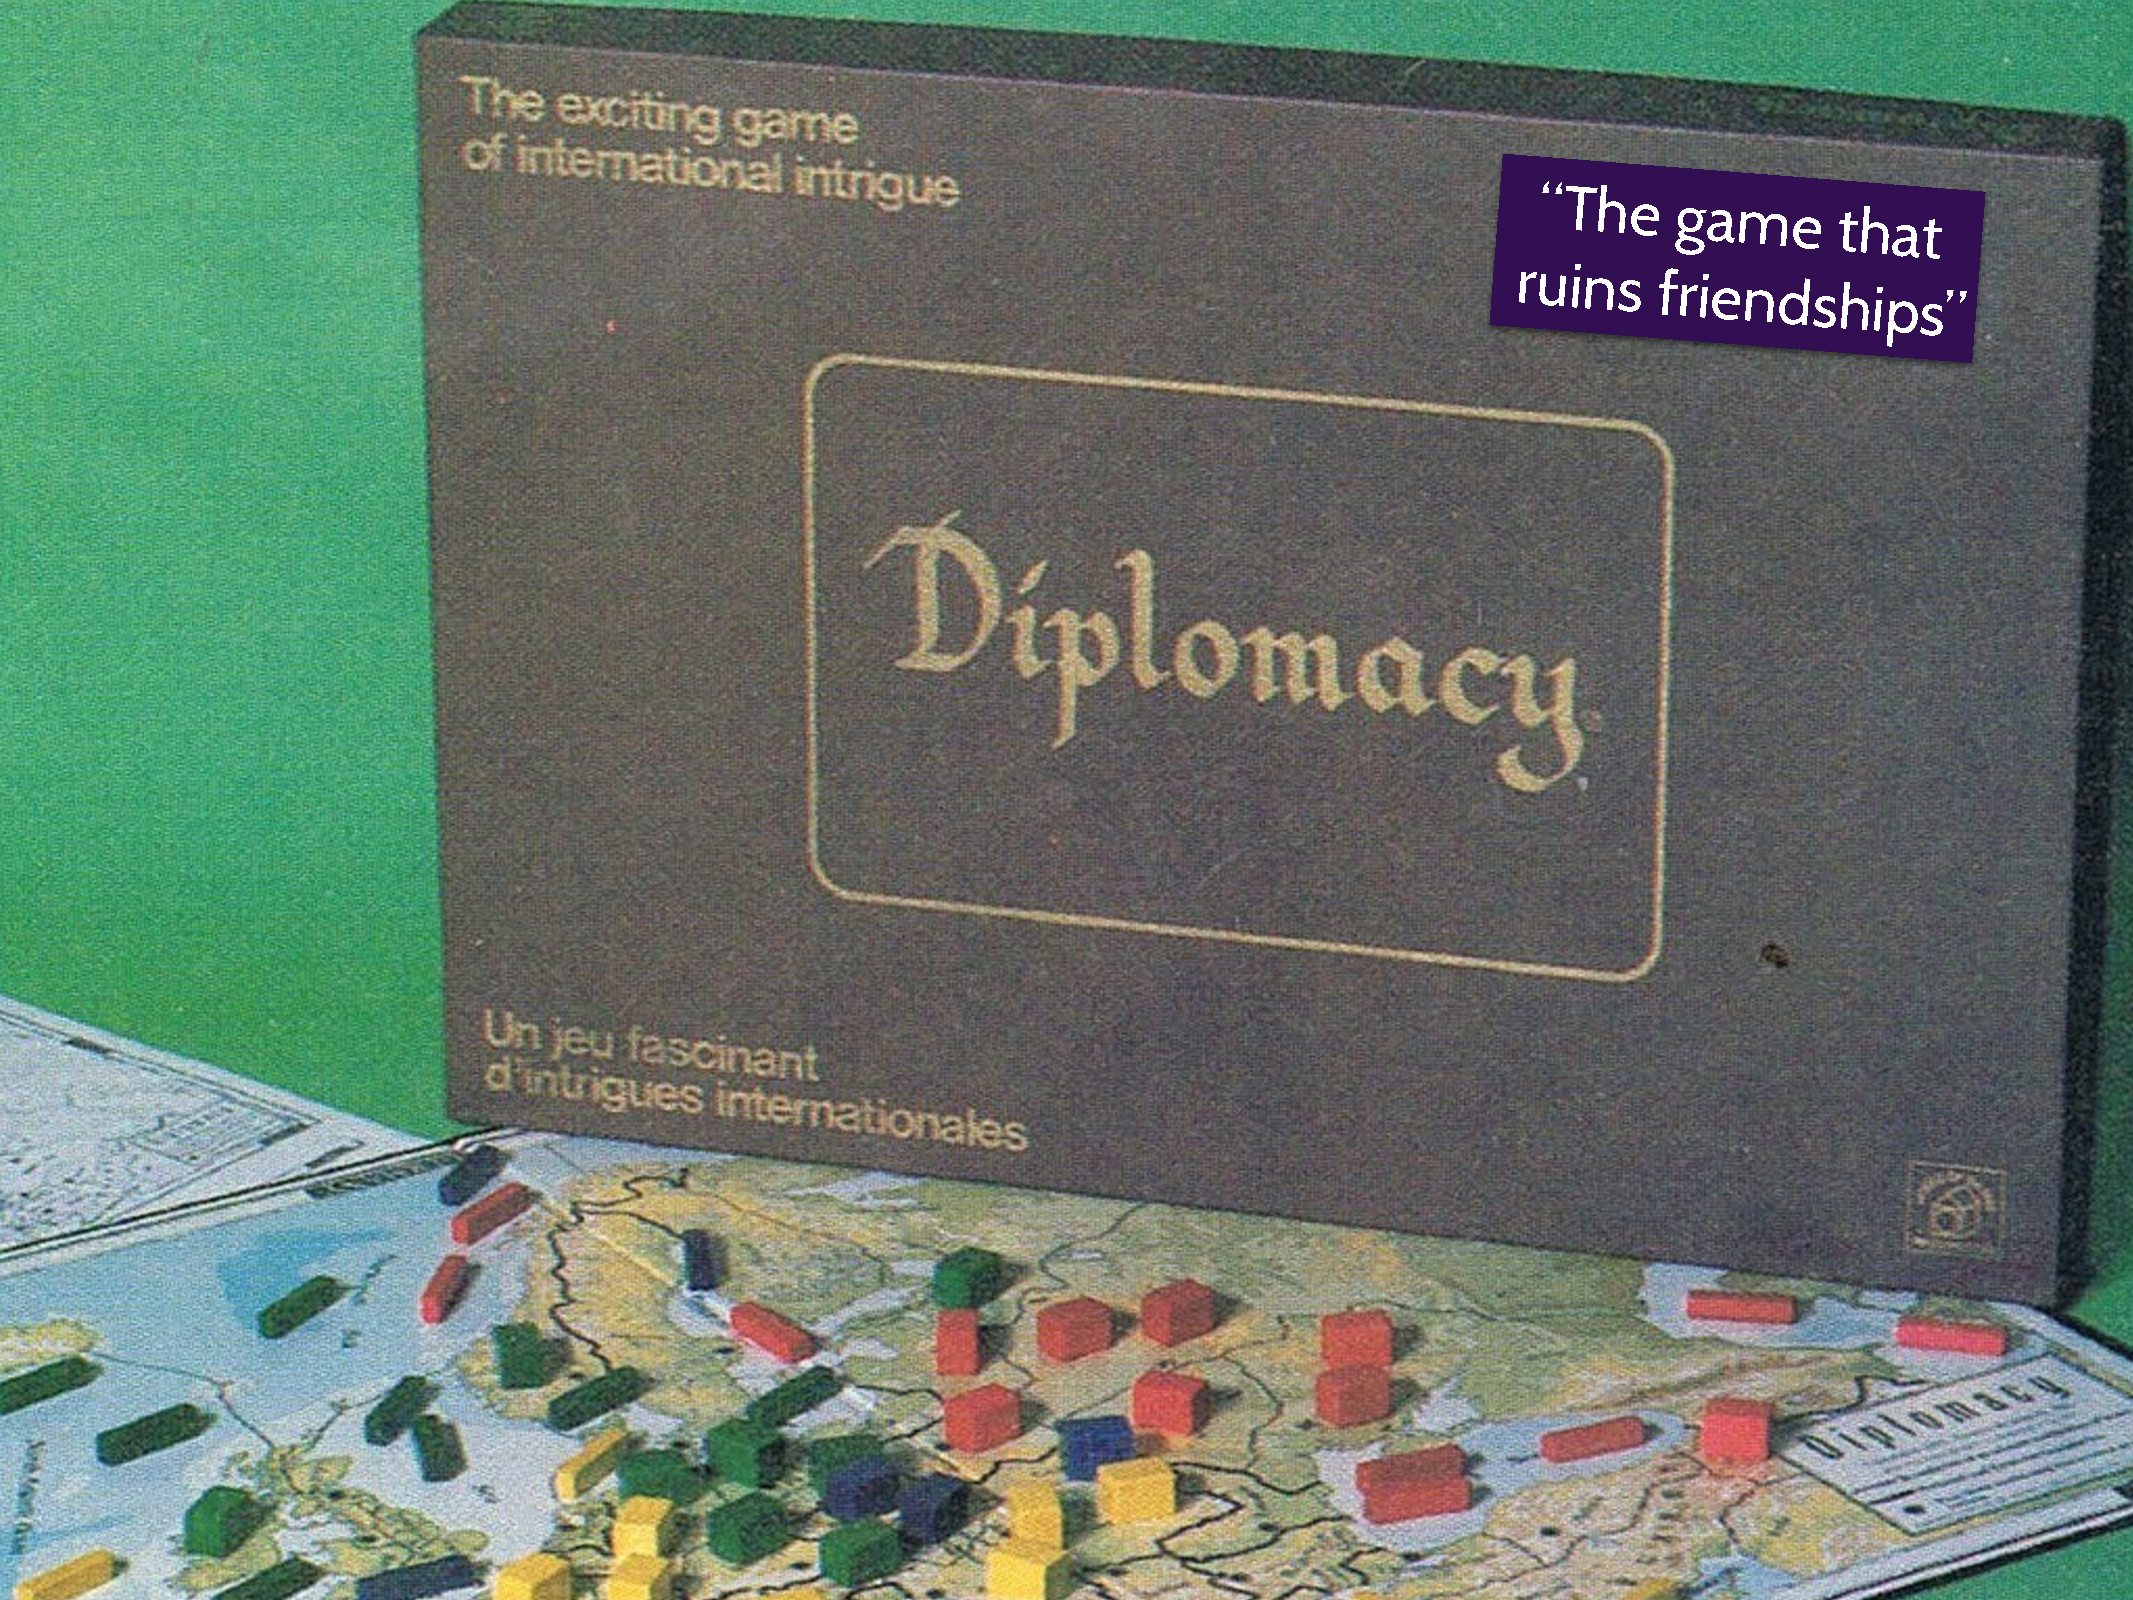
\includegraphics[page=1,width=\paperwidth]{diplomacy/betrayal-slides}}}
	\only<2>{\makebox[\linewidth]{\includegraphics[page=2,width=\paperwidth]{diplomacy/betrayal-slides}}}
	\only<3>{\makebox[\linewidth]{\includegraphics[page=3,width=\paperwidth]{diplomacy/betrayal-slides}}}
	\only<4>{\makebox[\linewidth]{\includegraphics[page=4,width=\paperwidth]{diplomacy/betrayal-slides}}}
	\only<5>{\makebox[\linewidth]{\includegraphics[page=5,width=\paperwidth]{diplomacy/betrayal-slides}}}
	\only<6>{\makebox[\linewidth]{\includegraphics[page=6,width=\paperwidth]{diplomacy/betrayal-slides}}}
	\only<7>{\makebox[\linewidth]{\includegraphics[page=7,width=\paperwidth]{diplomacy/betrayal-slides}}}
	\only<8>{\makebox[\linewidth]{\includegraphics[page=8,width=\paperwidth]{diplomacy/betrayal-slides}}}
	\only<9>{\makebox[\linewidth]{\includegraphics[page=9,width=\paperwidth]{diplomacy/betrayal-slides}}}
	\only<10>{\makebox[\linewidth]{\includegraphics[page=10,width=\paperwidth]{diplomacy/betrayal-slides}}}
	\only<11>{\makebox[\linewidth]{\includegraphics[page=11,width=\paperwidth]{diplomacy/betrayal-slides}}}
	\only<12>{\makebox[\linewidth]{\includegraphics[page=12,width=\paperwidth]{diplomacy/betrayal-slides}}}
	\only<13>{\makebox[\linewidth]{\includegraphics[page=13,width=\paperwidth]{diplomacy/betrayal-slides}}}
	\only<14>{\makebox[\linewidth]{\includegraphics[page=14,width=\paperwidth]{diplomacy/betrayal-slides}}}
	\only<15>{\makebox[\linewidth]{\includegraphics[page=15,width=\paperwidth]{diplomacy/betrayal-slides}}}
	\only<16>{\makebox[\linewidth]{\includegraphics[page=16,width=\paperwidth]{diplomacy/betrayal-slides}}}
	\only<17>{\makebox[\linewidth]{\includegraphics[page=17,width=\paperwidth]{diplomacy/betrayal-slides}}}
	\only<18>{\makebox[\linewidth]{\includegraphics[page=18,width=\paperwidth]{diplomacy/betrayal-slides}}}
	\only<19>{\makebox[\linewidth]{\includegraphics[page=19,width=\paperwidth]{diplomacy/betrayal-slides}}}
	\only<20>{\makebox[\linewidth]{\includegraphics[page=20,width=\paperwidth]{diplomacy/betrayal-slides}}}
	\only<21>{\makebox[\linewidth]{\includegraphics[page=21,width=\paperwidth]{diplomacy/betrayal-slides}}}
\end{frame}

%TODO(jbg): Add Joy slide

\begin{frame}{Cicero is really good}
	\begin{columns}
		\column{.7\linewidth}
		\gfxd{cicero_model}{1.0}
		\column{.7\linewidth}
		\gfxd{cicero_results}{1.0}
	\end{columns}
	And we confirm their results, it wins around 90\% of games!
\end{frame}

\begin{frame}{}
	\begin{columns}
		\column{.5\linewidth}
		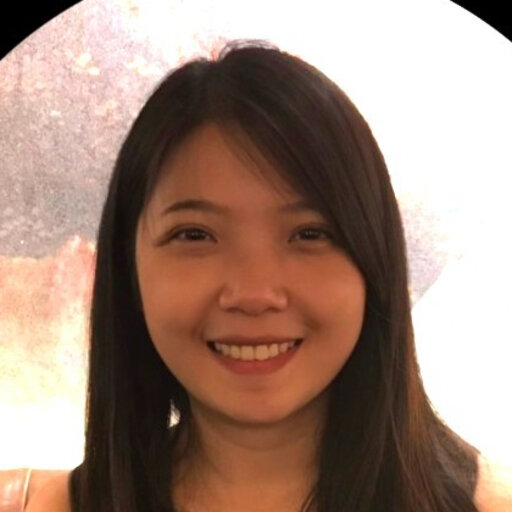
\includegraphics[width=1.0\linewidth]{general_figures/joy}
		\column{.5\linewidth}
		\gfxd{benchmark_paper}{1.0}
	\end{columns}
\end{frame}

\begin{frame}{Can they tell it's a bot?}
	\begin{columns}
		\column{.5\linewidth}
		\begin{block}{Passing the Turing Test?}
			No in-game messages indicated that players believed they were playing with an AI agent. One player mentioned in post-game chat a suspicion that one of Cicero’s accounts might be a bot, but this did not lead to Cicero being detected as an AI agent by other players in the league.
		\end{block}
		\column{.5\linewidth}
		\only<1>{\gfxd{benchmark_detection_0}{.9}}
		\only<2>{\gfxd{benchmark_detection_1}{.9}}
		\only<3>{\gfxd{benchmark_detection_2}{.9}}
		\only<4>{\gfxd{benchmark_detection_3}{.9}}
	\end{columns}
\end{frame}

\begin{frame}{Persuasion}
	\only<1>{\gfxd{persuasion}{.15}}
	\only<2>{\gfxd{persuasion_1}{.8}}
	\only<3>{\gfxd{persuasion_2}{.8}}
	\only<4>{\gfxd{persuasion_3}{.8}}
	\only<5>{\gfxd{persuasion_4}{.8}}
\end{frame}


\begin{frame}{People Think Cicero Lies More}
	\gfxd{percieved_lies}{.8}
\end{frame}

\begin{frame}{Broken Commitments (subset of deception)}
	\only<1>{\gfxd{cicero_deception_1}{.25}}
	\only<2>{\gfxd{cicero_deception_2}{.4}}
	\only<3>{\gfxd{cicero_deception_3}{.6}}
\only<4>{\gfxd{cicero_deception_4}{0.75}}	
\end{frame}

\begin{frame}{People Lie to Cicero More}
	\gfxd{lies_sent}{.8}
\end{frame}

\begin{frame}{}
	\begin{columns}
		\column{.5\linewidth}
		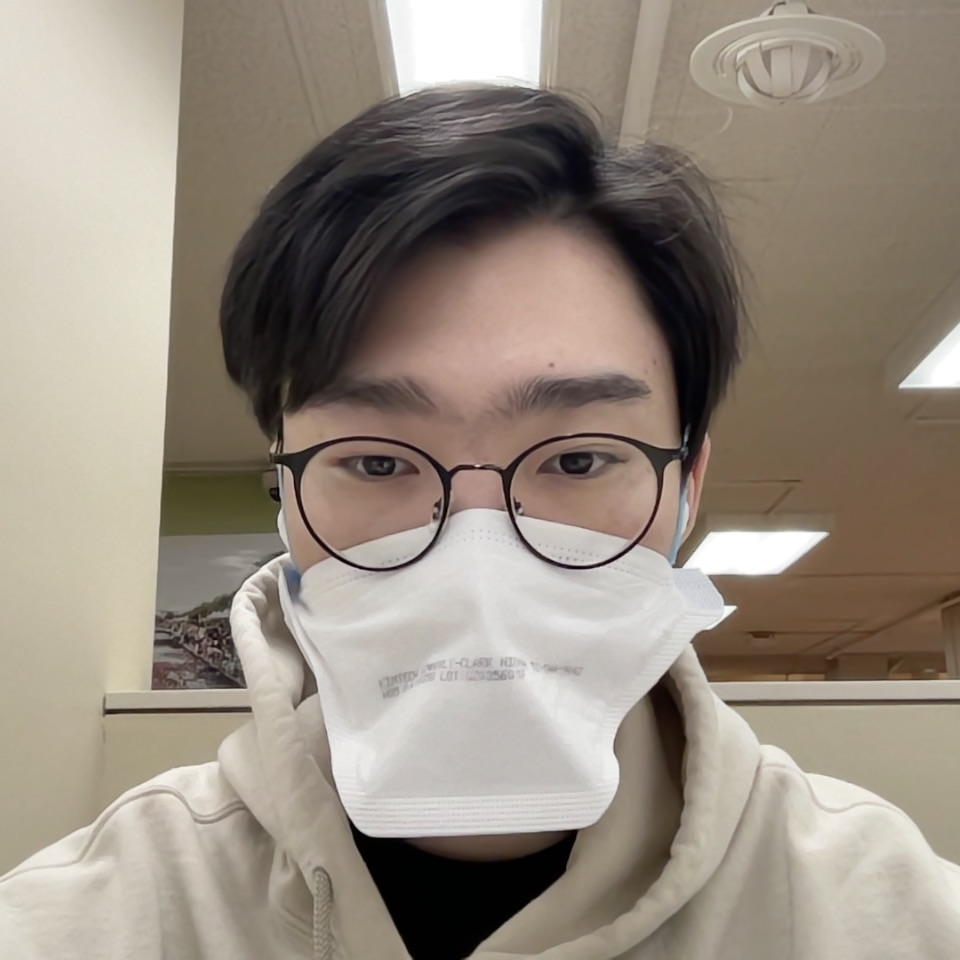
\includegraphics[width=1.0\linewidth]{general_figures/feng}
		\column{.5\linewidth}
		\gfxd{pholus_paper}{1.0}
	\end{columns}
\end{frame}


\begin{frame}{Giving Advice}
	\only<1>{\gfxd{pholus_interface}{1.0}}
	\only<2>{\gfxd{pholus_interface_label}{1.0}}
\end{frame}

\begin{frame}{Advice Helps}
	\only<1>{\gfxd{chiron_skill_regression}{.5}\gfxd{pholus_coefficient_scale}{.5}}
	\only<2>{\gfxd{chiron_all_regression}{.5}}
		
	\only<3>{\gfxd{chiron_acceptance}{.5}}

\end{frame}

\begin{frame}{How to better detect Deception}
	\only<1>{\gfxd{pholus_map}{.5}}
	\only<2>{\gfxd{pholus_map_1}{.6}}	
	\only<3>{\gfxd{pholus_map_2}{1.0}}	
	\only<4>{\gfxd{pholus_map_3}{1.0}}
	\only<5>{\gfxd{pholus_map_4}{1.0}}
	
\end{frame}

\begin{frame}{It's Time for Some Game Theory}
	\only<1>{\gfxd{pholus_grid_0}{1.0}}
	\only<2>{\gfxd{pholus_grid_1}{1.0}}
	\only<3>{\gfxd{pholus_grid_2}{1.0}}
	\only<4>{\gfxd{pholus_grid_3}{1.0}}
	\only<5>{\gfxd{pholus_grid_4}{1.0}}	
\end{frame}

\begin{frame}{Really Hard Problem, but Better}
	\gfxd{pholus_deception_detection}{.7}
	
	Human ability is around 0.2
\end{frame}

\begin{frame}{Recap}
	\begin{itemize}
		\item Reinforcement learning is really good at determining moves
		\item Language and cooperation lags behind
		\item Diplomacy remains a useful language game
		\begin{itemize}
			\item Not just for winning the game
			\item Are you respected
			\item Are you truthful
			\item Are you helpful
		\end{itemize}
		\item Maybe we can do this on a small scale so that it applies to all \abr{ai}
	\end{itemize}
	
\end{frame}

\begin{frame}{Human and Computer Skills}
	\begin{itemize}
	\item LLMs are not perfect
	\begin{itemize}
		\item Retrieval Methods: Slow but Trustworthy
		\item LLMs: Use if you are confident
		\item Humans: Leave them in driver's seat
	\end{itemize}
	\item Item Response Theory
	\begin{itemize}
		\item Highlight skills and examples
		\item Measure how much computers \emph{help} or \emph{hurt}
	\end{itemize}
	\item Application
	\begin{itemize}
		\item Supporting Users to find False Claims
		\item Supporting Users to Answer Questions
		\item Supporting Users to Negotiate
	\end{itemize}
	\end{itemize}
\end{frame}

\begin{frame}{Why didn't you\dots}
  \begin{itemize}
  \item IR works better than LLM for fact checking \emph{sometimes}
  \item We also showed bandit model can figure out what evidence to show when
  \item Use Bandit model to show \emph{right} evidence to user
    \pause
  \item We're trying\dots requires good calibration
  \item ACL Submission: Adversarial Calibration
  \item Looking for collaborators
  \end{itemize}
\end{frame}

\fsi{general_figures/black_box_outline}{}
\fsi{general_figures/kill_all_humans}{}
\fsi{general_figures/blackbox}{}
%\fsi{general_figures/bennet_robot}{}
\fsi{general_figures/tng_poker}{}




\frame{
	
	\frametitle{Thanks}
	
	%TODO(jbg): Check 
	\begin{block}{Collaborators}
		Hal Daum\'e III (UMD), Jon May (USC), Cristian (Columbia), Marine Carpuat
		(UMD), Eve Fleisig (Berkeley), Sherry Wu (CMU)
	\end{block}
	
	\begin{columns}
		
		\column{.75\linewidth}
		\begin{block}{Funders}
			\begin{center}
				
\includegraphics[width=0.2\linewidth]{general_figures/nsf}
				
\includegraphics[width=0.2\linewidth]{general_figures/darpa}
				
\includegraphics[width=0.2\linewidth]{general_figures/arl}
				
\includegraphics[width=0.2\linewidth]{general_figures/iarpa}
			\end{center}
		\end{block}
		
		\column{.3\linewidth}
		\begin{block}{Supporters}
			
\includegraphics[width=1.0\linewidth]{general_figures/iac}
			\gfxq{naqt}{1.0}
		\end{block}
		
	\end{columns}
}





\begin{frame}{Moving beyond games}

  \begin{columns}
    \column{.5\linewidth}
  \begin{itemize}
    \item Exhausting for humans
    \item Computers not trusted
    \item Differential strengths
    \item Same word-by-word characteristic
  \end{itemize}

  \column{.5\linewidth}
 \gfxs{computer-interpreter}{1.0}
 \end{columns}
\end{frame}


\begin{frame}{}
  \begin{columns}
    \column{.2\linewidth}
    \begin{center}
        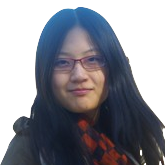
\includegraphics[width=0.8\linewidth]{general_figures/hehe} \\
        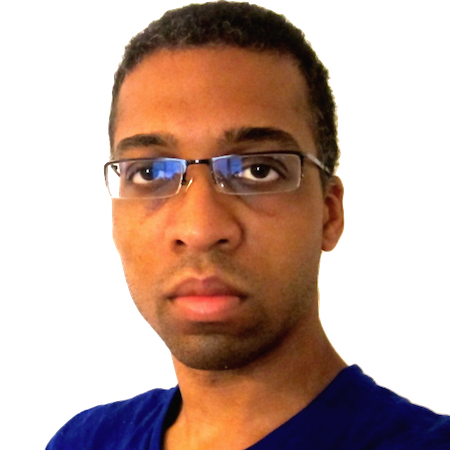
\includegraphics[width=0.8\linewidth]{general_figures/alvin}
        \\
        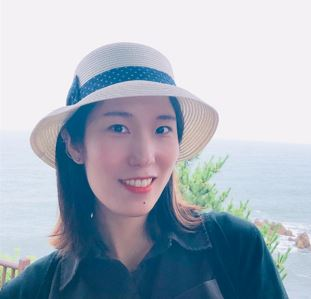
\includegraphics[width=0.8\linewidth]{general_figures/hyojung}
        \end{center}
    \column{.8\linewidth}

        \begin{block}{ {\bf
              \href{http://umiacs.umd.edu/~jbg//docs/2014_emnlp_simtrans.pdf}{Don’t Until the Final Verb Wait: Reinforcement Learning for Simultaneous Machine Translation}}}
          \small
Alvin Grissom II, He He, {\bf Jordan Boyd-Graber}, John Morgan, and Hal {Daum\'{e} III}.  \emph{Empirical Methods in Natural Language Processing}, 2014
        \end{block}

        \begin{block}{ {\bf
              \href{http://umiacs.umd.edu/~jbg/docs/2016_naacl_interpretese.pdf}{Interpretese
                vs. Translationese: The Uniqueness of Human Strategies
                in Simultaneous Interpretation}}}
          \small
He He, {\bf Jordan Boyd-Graber}, and Hal {Daum\'{e} III}.
\emph{North American Association for Computational Linguistics}, 2016
        \end{block}


        \begin{block}{ {\bf
              \href{http://umiacs.umd.edu/~jbg/docs/2022_emnlp_simint.pdf}{SimQA:
                Detecting Simultaneous MT Errors through 
                Word-by-Word Question Answering}}}
          \small
          \href{https://h-j-han.github.io/}{HyoJung Han}, Marine
            Carpuat, {\bf Jordan Boyd-Graber}.  \emph{Empirical Methods in Natural Language Processing}, 2022
          
          \end{block}
  \end{columns}


\end{frame}



\fsi{simtrans/liang_huang}{}
\fsi{simtrans/delay}{}

\begin{frame}{How to Evaluate}

  \begin{columns}
    \column{.5\linewidth}
    \only<1>{
      
\includegraphics[width=1.0\linewidth]{simtrans/polish_jeopardy}}
    \only<2->{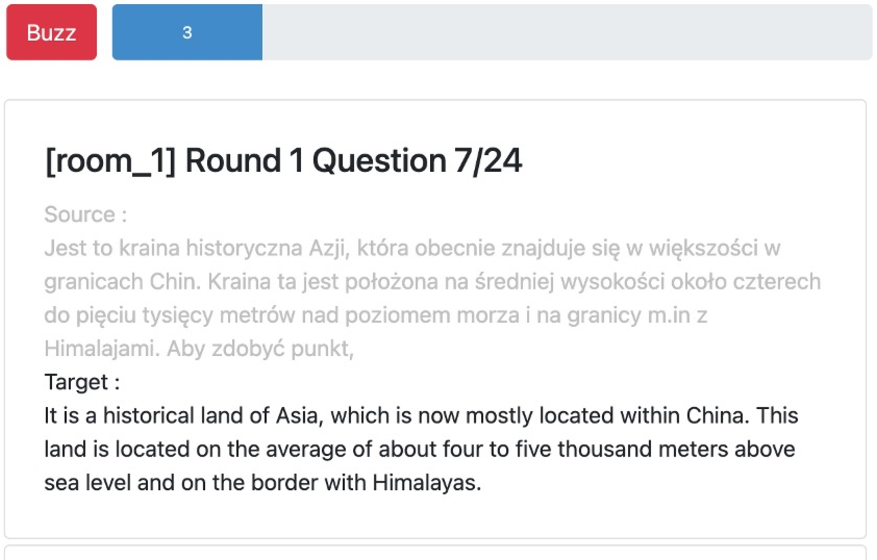
\includegraphics[width=0.8\linewidth]{simtrans/interface}}
    \column{.5\linewidth}
    \begin{itemize}
    \item You're a contestant on a Polish game show
    \item You have access to a simultaneous translation system
    \item Your job is to answer the question before your opponent (as
      quickly as possible)
      \only<3>{\alert<3>{ \item Keep question answerer the same, vary translation}}
    \end{itemize}
  \end{columns}

\end{frame}

\begin{frame}{BLEU results for modern Simultaneous Translation Systems}

  \begin{center}
  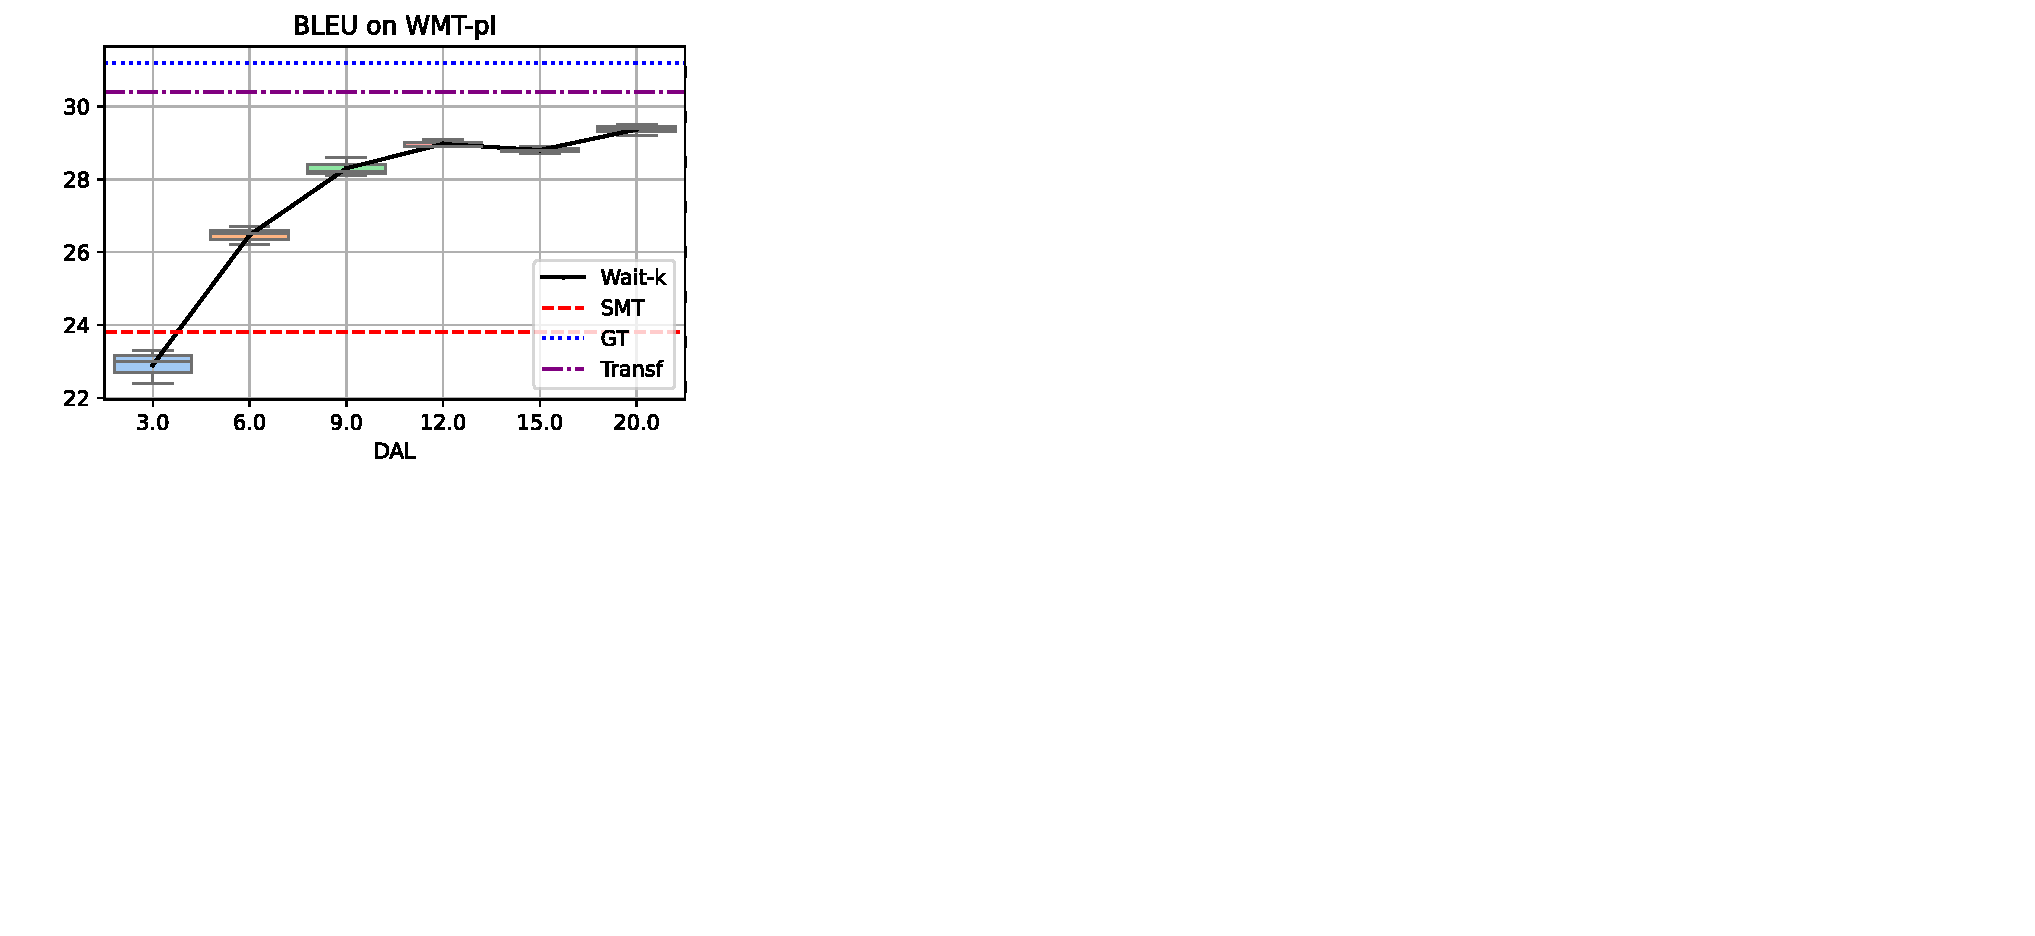
\includegraphics[width=0.9\linewidth]{simtrans/simQA/bleu_simqa}
\end{center}

\end{frame}

\begin{frame}{Downstream QA Results}

  \begin{center}
  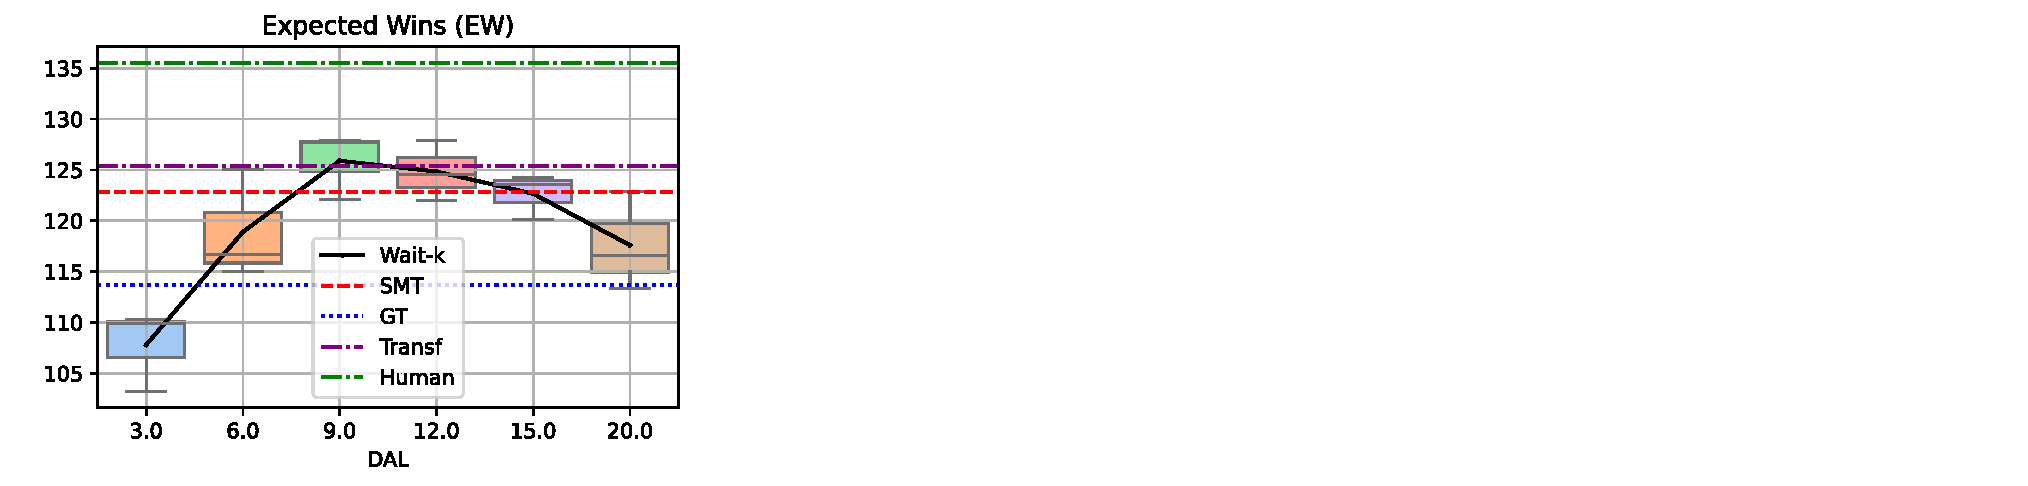
\includegraphics[width=0.8\linewidth]{simtrans/simQA/qametrics_simqa}
\end{center}

\only<2->{Additional benefit: Only need to translate the answer}

\end{frame}


\begin{frame}{Undertranslation}
  \begin{center}
    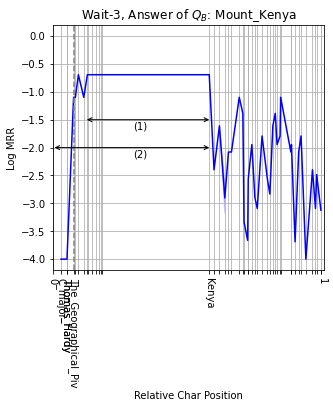
\includegraphics[width=0.4\paperwidth]{simtrans/simQA/ex_undertranslation}
  \end{center}
When the translation doesn't
help\dots
\end{frame}

\begin{frame}{When are Mistakes / Hallucinations Harmful?}


  \begin{center}
    \only<2->{This coordinate determines}
    \only<3->{the double-wall}
    \only<4->{angle between the southern half of the meridian plane
      and the}
    \only<5->{southern}
  \only<1>{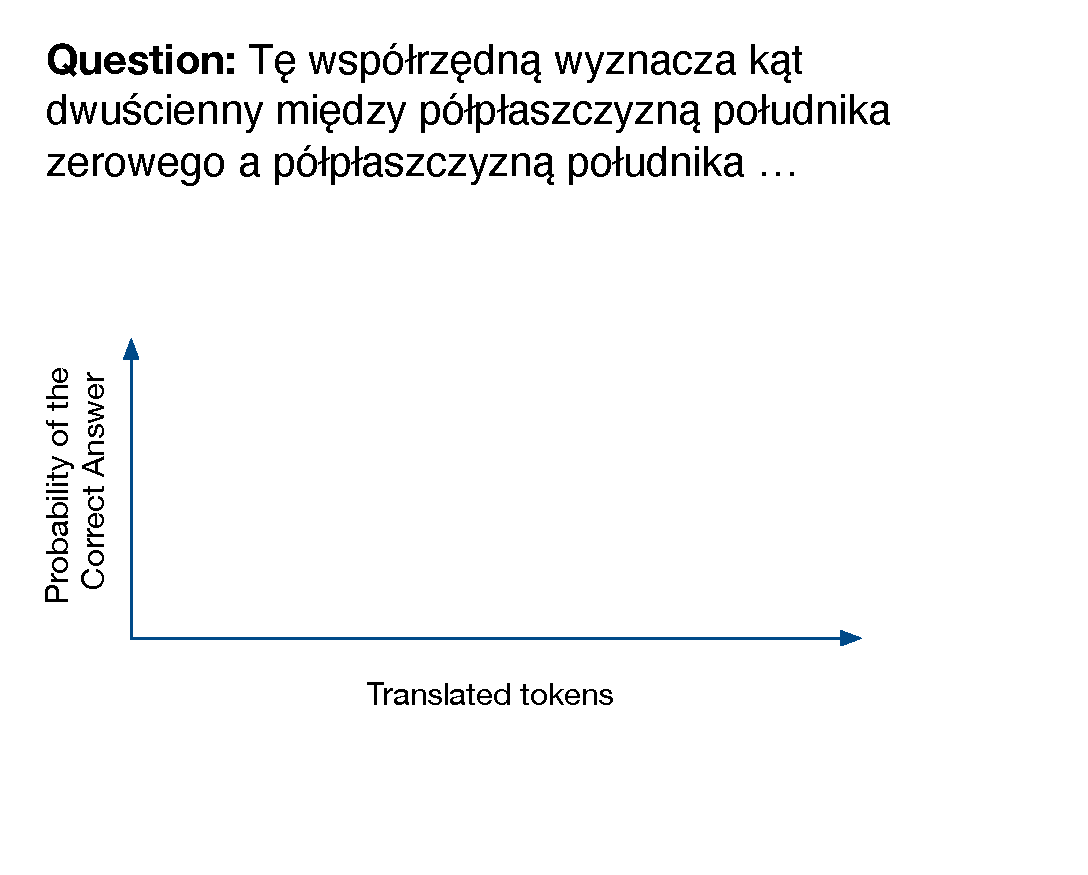
\includegraphics[width=0.5\paperwidth]{simtrans/simQA/hallucination_example_0}}
  \only<2>{\includegraphics[width=0.5\paperwidth]{simtrans/simQA/hallucination_example_1}}
  \only<3>{\includegraphics[width=0.5\paperwidth]{simtrans/simQA/hallucination_example_2}}
  \only<4>{\includegraphics[width=0.5\paperwidth]{simtrans/simQA/hallucination_example_5}}  
  \only<5>{\includegraphics[width=0.5\paperwidth]{simtrans/simQA/hallucination_example_3}}
  \only<6>{\includegraphics[width=0.5\paperwidth]{simtrans/simQA/hallucination_example_4}}
\end{center}
{\bf Guess: } \only<1>{??} \only<2>{IP Address} \only<3>{Spherical
  Coordinate} \only<4>{Longitude} \only<5>{Spherical Coordinate} \only<6>{Longitude}
\end{frame}



\frame{
  \frametitle{But wait, there's more!}

  \vspace{-.5cm}

\begin{columns}



  \column{.5\linewidth}

   \begin{block}{Computational Social Science}
     \centering
     \includegraphics[width=0.8\linewidth]{teaparty/figures/framing} \\
     \cite{nguyen-13b,nguyen-15}
   \end{block}


    \begin{block}{Detecting Deception}
    \centering
        \includegraphics[width=0.4\linewidth]{general_figures/diplomacy} \\
        \cite{peskov-20,Eisenschlos-21}
    \end{block}

  \column{.5\linewidth}


    \begin{block}{Multilingual/Multicultural Models}
      \begin{center}
        \includegraphics[width=0.4\linewidth]{general_figures/tonal_translation} \\
      \cite{hu-14,Guo-22}
       \end{center}
    \vspace{-.3cm}
    \end{block}


  \begin{block}{Computational Biology}
     \centering
     \includegraphics[width=0.4\linewidth]{general_figures/protein} \\
     \small
     \cite{nguyen-13b,hu-13:coalescent}
   \end{block}





\end{columns}

}


\frame{

\begin{columns}

\column{.5\linewidth}

\includegraphics[width=.8\linewidth]{general_figures/forough}

\column{.5\linewidth}

\begin{block}{ALTO: Active Learning with Topic Overviews for Speeding Label Induction and Document Labeling}
Forough Poursabzi-Sangdeh, Jordan Boyd-Graber, Leah Findlater, and Kevin Seppi.  Association for Computational Linguistics, 2016.
\end{block}

\end{columns}

}



\fsi{interactive_topic_models/alto_interface}{}
\fsi{interactive_topic_models/alto_interface_highlight}{Direct users
  to document}



\fsi{interactive_topic_models/alto/user_talk_1}{ Active learning if time is short}
\fsi{interactive_topic_models/alto/user_talk_2}{ Better than status quo}
\fsi{interactive_topic_models/alto/user_talk_3}{ Active learning can
  help topic models }
\fsi{interactive_topic_models/alto/user_talk_4}{ Topic models help
  users understand the collection }
\fsi{interactive_topic_models/alto/user_talk_4}{ Moral: machines and
  humans together (if you let them) }


\fsi{qb/viz_first_draft}{Andrea Lin}



\fsi{simtrans/liang_huang}{}
\fsi{simtrans/delay}{}

\begin{frame}{How to Evaluate}

  \begin{columns}
    \column{.5\linewidth}
    \only<1>{
      \includegraphics[width=1.0\linewidth]{simtrans/polish_jeopardy}}
    \only<2->{\includegraphics[width=0.8\linewidth]{simtrans/interface}}
    \column{.5\linewidth}
    \begin{itemize}
    \item You're a contestant on a Polish game show
    \item You have access to a simultaneous translation system
    \item Your job is to answer the question before your opponent (as
      quickly as possible)
      \only<3>{\alert<3>{ \item Keep question answerer the same, vary translation}}
    \end{itemize}
  \end{columns}

\end{frame}

\begin{frame}{BLEU results for modern Simultaneous Translation Systems}

  \begin{center}
  \includegraphics[width=0.9\linewidth]{simtrans/simQA/bleu_simqa}
\end{center}

\end{frame}

\begin{frame}{Downstream QA Results}

  \begin{center}
  \includegraphics[width=0.8\linewidth]{simtrans/simQA/qametrics_simqa}
\end{center}

\only<2->{Additional benefit: Only need to translate the answer}

\end{frame}


\begin{frame}{Undertranslation}
  \begin{center}
    \includegraphics[width=0.4\paperwidth]{simtrans/simQA/ex_undertranslation}
  \end{center}
When the translation doesn't
help\dots
\end{frame}

\begin{frame}{When are Mistakes / Hallucinations Harmful?}


  \begin{center}
    \only<2->{This coordinate determines}
    \only<3->{the double-wall}
    \only<4->{angle between the southern half of the meridian plane
      and the}
    \only<5->{southern}
  \only<1>{\includegraphics[width=0.5\paperwidth]{simtrans/simQA/hallucination_example_0}}
  \only<2>{\includegraphics[width=0.5\paperwidth]{simtrans/simQA/hallucination_example_1}}
  \only<3>{\includegraphics[width=0.5\paperwidth]{simtrans/simQA/hallucination_example_2}}
  \only<4>{\includegraphics[width=0.5\paperwidth]{simtrans/simQA/hallucination_example_5}}  
  \only<5>{\includegraphics[width=0.5\paperwidth]{simtrans/simQA/hallucination_example_3}}
  \only<6>{\includegraphics[width=0.5\paperwidth]{simtrans/simQA/hallucination_example_4}}
\end{center}
{\bf Guess: } \only<1>{??} \only<2>{IP Address} \only<3>{Spherical
  Coordinate} \only<4>{Longitude} \only<5>{Spherical Coordinate} \only<6>{Longitude}
\end{frame}


\begin{frame}{References}
\bibliographystyle{style/acl}
\tiny
\bibliography{bib/journal-full,bib/jbg,bib/hhe,bib/alvin,teaparty/vietan,bib/hoyle}
\end{frame}




\begin{frame}{Calibration is hard}
	
	\begin{itemize}
		\item If they knew when they were making stuff up, this wouldn’t be a problem
		But LLMs are notoriously bad at knowing when they don’t know
		\begin{itemize}
			\item Depends on length of generation
			\item Depends on frequency of response
			\item Depends on reasoning
			\item Depends on tokenization 
		\end{itemize}
		\item Even our metrics for knowing when the uncertainty is bad are flawed
		\item And doing a good job of detection requires deeper access to the model
	\end{itemize}
\end{frame}



\begin{frame}{The Value of Repeated Games}

  \begin{itemize}
  \item We're only learning per example
  \item Can we learn more efficiently?
  \item What if we got feedback per token?
    \pause
    \begin{itemize}
      \item Improve Calibration
      \item Improve Cooperation
    \end{itemize}
  \end{itemize}

\end{frame}

\begin{frame}{Human--Computer Calibration}
	\begin{columns}
		\column{.4\linewidth}
		\begin{itemize}
			\item Questions get easier
			(for humans)
			\item Humans evaluate whether they know enough to answer
			\item If they answer too early, they get “locked out” from the rest of the questions
			\item Big idea: what if we give the humans tools to better understand computer thought process
			
		\end{itemize}
		
		\column{.6\linewidth}
		\gfxq{example_game}{1.0}
	\end{columns}
	
\end{frame}

\begin{frame}[plain]
  \vspace{-2cm}
		\includegraphics[width=1.0\linewidth]{qb/jeopardy}
                \pause
                \vspace{-8cm}
         \begin{block}{This is {\bf not} Jeopardy}
		\begin{itemize}
                        \item Jeopardy: must decide to answer {\bf once}, after
                          complete question
                        \item Quiz Bowl: decide after each word
		\end{itemize}

	\end{block}

\end{frame}




% TODO add more questions here

\begin{frame}[t]
\frametitle{Sample Question}
	\frametitle{Sample Question}

With Leo Szilard, he invented a doubly-eponymous \only<2->{refrigerator with no moving parts. He did not take interaction with neighbors into account when formulating his theory of} \only<3->{heat capacity, so} \only<4->{Debye adjusted the theory for low temperatures. His} \only<4->{summation convention automatically sums repeated indices in tensor products. His name is attached to the A and B coefficients} \only<5->{for spontaneous and stimulated emission, the subject of one of his multiple groundbreaking 1905 papers. He further developed the model of statistics sent to him by} \only<6->{Bose to describe particles with integer spin. For 10 points, who is this German physicist best known for formulating the} \only<7->{special and general theories of relativity?} \\
\vspace{1cm}
\only<8->{ {\bf Albert \underline{Einstein}}}

\only<9->{
\vspace{-6cm}

\begin{block}{Faster = Smarter, More Calibrated}

  \begin{enumerate}
    \item University of Chicago
    \item Colorado School of Mines
    \item Cornell University
    \item UIUC
    \item Brigham Young University
    \item California Institute of Technology
    \item Peking University
    \item Harvey Mudd College
    \item Darmstadt University
    \item University of Colorado
  \end{enumerate}


\end{block}
}

\end{frame}


% \begin{frame}[t]
% 	\frametitle{Sample Question}

%         The Swiss-Italian architect Pietro Antonio Solari
%         \only<2->{built several fortified towers in this city, which
%           often vied for power with its northern rival Tver. A ruler
%           of this city prevailed in the} \only<3->{Great Stand on the
%           Ugra River. A prince from this city was nicknamed for
%           winning a battle on the} \only<4->{Don river. Partly because
%           a ruler of this city married} \only<5->{Sophia Palaiologina,
%           the niece of the last Byzantine Emperor, this city styled
%           itself the} \only<6->{``Third Rome'' after the fall of
%           Constantinople. Another prince of this city stopped paying
%           tribute to the} \only<7->{Mongols in 1476, ending the
%           ``Tatar yoke.''} \only<8->{The Grand Duchy headquartered in
%           this city came to an end in 1547 with the ascension of}
%         \only<9->{ Ivan IV, who made it his capital. For 10 points,
%           name this city where Ivan III renovated the
%           Kremlin,} \only<10->{the capital of Russia.}\\
%         \vspace{.5cm} \only<11->{ {\bf Moscow} (Moskva / Muscovy)}



% \end{frame}

% TODO: Diplomacy slides

% TODO: Chenglei slides

\begin{frame}{How does a computer buzz in?}

  \begin{itemize}
  \item Ask computer for guess every $N$ words
  \item Compute average log probability
  \begin{itemize}
  \item Threshold on log probability of output
  \item Threshold chosen from TrickMe set
  \item Can do better!
  \end{itemize}
  \item Again, only have one chance to buzz
  \end{itemize}
\end{frame}

\begin{frame}{Human--Computer Competition}
  
  \begin{itemize}
  \item Top human team won
  \item Best computer team had \emph{much} higher accuracy
  \item Computers had strictly higher accuracy
  \item Humans had \emph{much} higher \textbf{conditional} accuracy
  \end{itemize}

  \begin{columns}
    \column{.5\linewidth}
    % TODO(jbg): add animation
    \gfxa{accuracy_plot}{1.0}

    \column{.5\linewidth}    
    \gfxa{p_buzz_correct_2}{1.0}
    
  \end{columns}

  
\end{frame}



\begin{frame}{What's hard for Computers}
	\only<1>{\gfxa{simplex_0}{.9}}
	\only<2>{\gfxa{simplex_1}{.9}}	
	\only<3>{\gfxa{simplex_2}{.9}}
	\only<4->{\gfxa{simplex_3}{.9}}

        \only<5>{\gfxa{caimira_objective}{.5}}
\end{frame}


\begin{frame}{Aside: Family Tree}

  \begin{columns}
    \column{.3\linewidth}

    \vspace{2cm}
    \begin{block}{Bradley-Terry Models}
\gfxq{rlhf}{1.0}
    \end{block}

    \column{.3\linewidth}
    \begin{block}{Zermelo}
\gfxq{Ernst_Zermelo_1900s}{0.5}
    \end{block}

    \begin{block}{Ideal Point Models}
\gfxq{dw_nominate}{1.0}
    \end{block}
    
    \column{.3\linewidth}    

    \vspace{2cm}
    \begin{block}{ELO Models}
\gfxq{elo}{1.0}
    \end{block}

    
  \end{columns}

  
\end{frame}



\begin{frame}{What more do we need?}
\only<1>{\gfxa{caimira_0}{.9}}
\only<2>{\gfxa{caimira_1}{.9}}
\only<3>{\gfxa{caimira_2}{.9}}
\only<4>{\gfxa{caimira_3}{.9}}
\only<5>{\gfxa{caimira_4}{.9}}
\end{frame}


\end{document}
